\begin{frame}{Added Captions!}
    \centering
    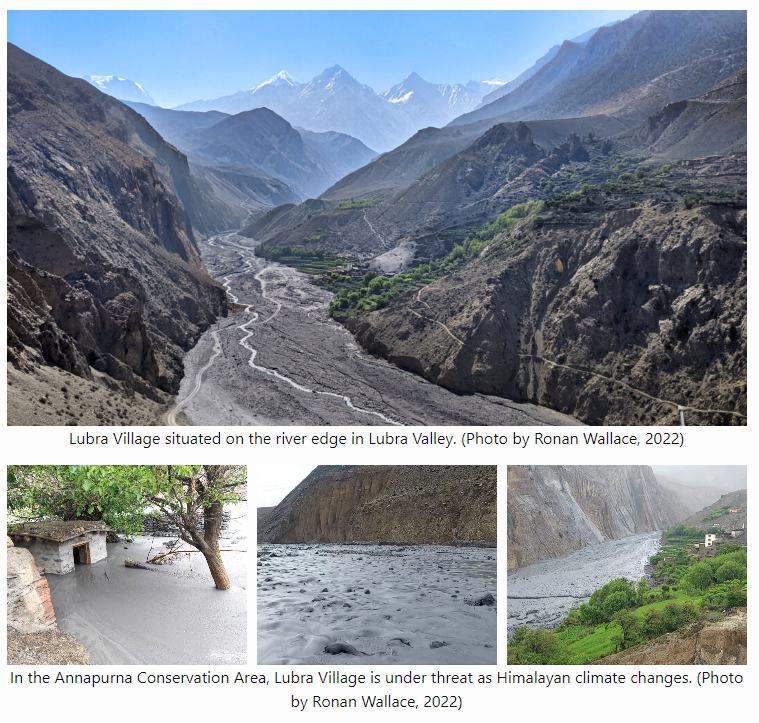
\includegraphics[height=0.7\textheight,width=0.7\textwidth,keepaspectratio]{images/Screenshot 2024-04-11 205424.png}
\end{frame}

\begin{frame}{Clean Up Projects... In Progress!}
    \begin{itemize}
        \item Verified images and links work 100\%
        \item Frist pass styling 90\%
        \item There are a few snags...
    \end{itemize}
\end{frame}

\begin{frame}{Added Captions!}
    \centering
    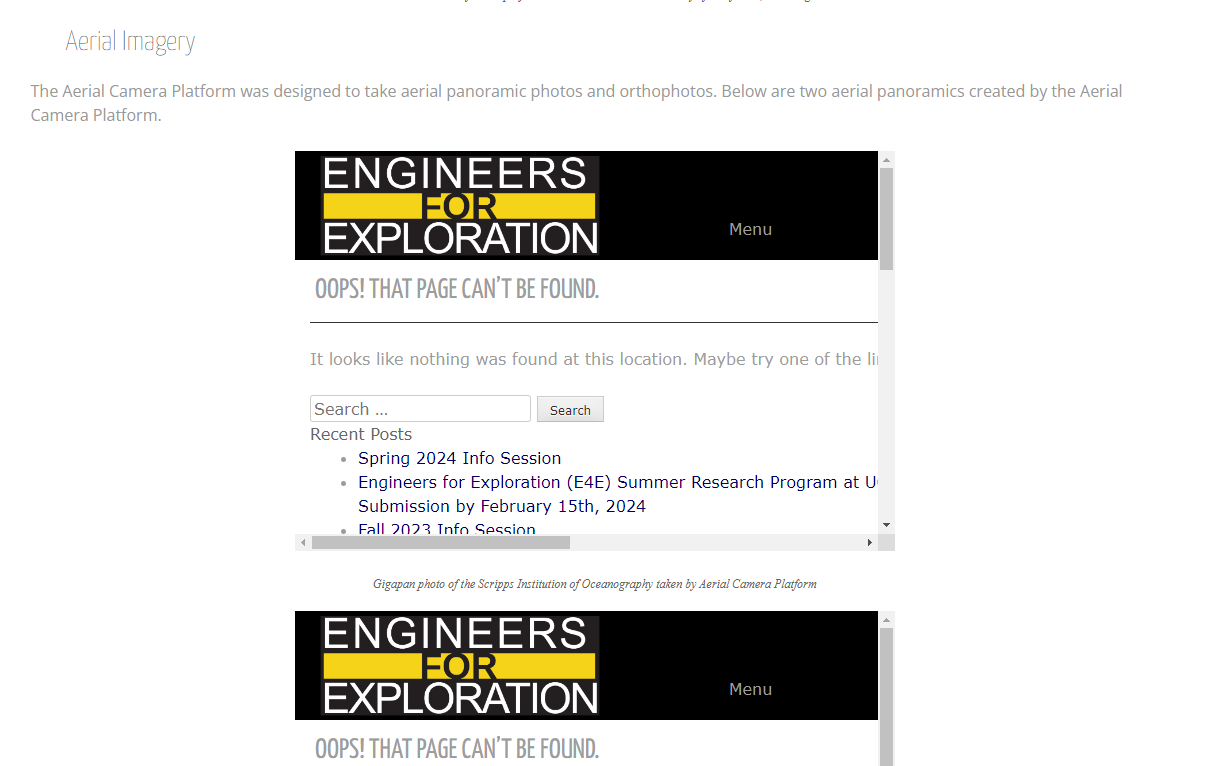
\includegraphics[height=0.7\textheight,width=0.7\textwidth,keepaspectratio]{images/dead_links.png}
\end{frame}

\begin{frame}{Dead Links in Current Site}
    \begin{itemize}
        \item https://e4e.ucsd.edu/stabilized-aerial-camera-platform contains 2 missing iframes
        \item https://e4e.ucsd.edu/vaquita doesn't exist
        \item In https://e4e.ucsd.edu/del-dios-monitoring, https://sdrvc.org/current/invasives-management/151 doesn't exist
        \item 4 other projects have missing external links
    \end{itemize}
\end{frame}

\begin{frame}{Remaining Styling: Maya Archaeology}
    \centering
    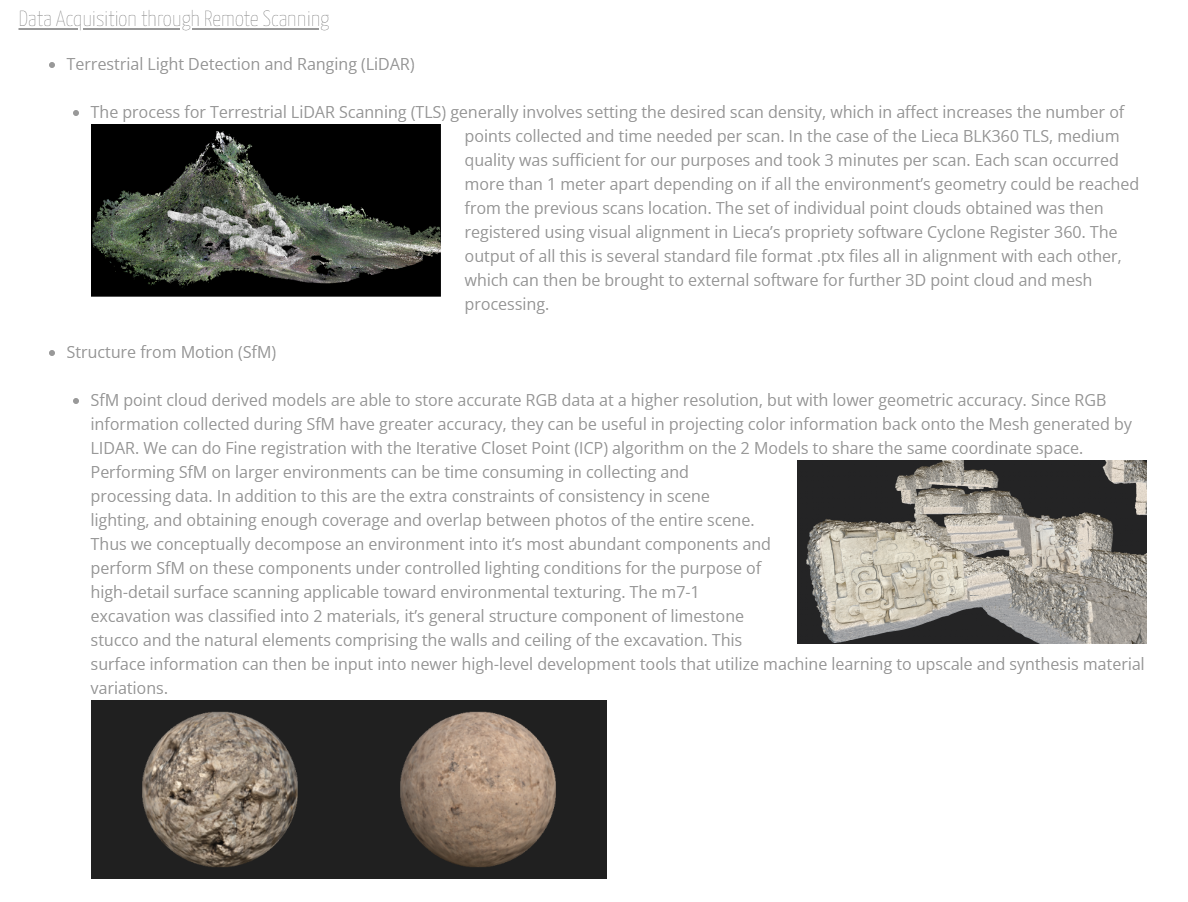
\includegraphics[height=0.7\textheight,width=0.7\textwidth,keepaspectratio]{images/maya.png}
\end{frame}




% Slides for 2024-04-12
% To create a slide, use the following:
% \begin{frame}{TITLE}
%     BODY
% \end{frame}

% To create a slide with a bullet list, use the following:
% \begin{frame}{TITLE}
%     \begin{itemize}
%         \item ITEM 1
%         \item ITEM 2
%     \end{itemize}    
% \end{frame}

% To create a slide with numbered list, use the following:
% \begin{frame}{TITLE}
%     \begin{enumerate}
%         \item ITEM 1
%         \item ITEM 2
%     \end{enumerate}
% \end{frame}

% To create a slide with a graphic:
% 1. Add the graphic to this folder (named picture.png)
% 2. Use the following:
% \begin{frame}{TITLE}
%     \centering
%     \includegraphics[height=0.7\textheight,width=0.7\textwidth,keepaspectratio]{picture.png}
% \end{frame}

% To create a slide with two columns, use the following:
% \begin{frame}{TITLE}
%     \begin{columns}
%         \begin{column}{0.5\textwidth}
%             COLUMN 1 BODY
%         \end{column}
%         \begin{column}{0.5\textwidth}
%             COLUMN 2 BODY
%         \end{column}
%     \end{columns}
% \end{frame}
